%% Unfolding and respective studies
\section{Correcting for detector effects}
\label{sec:unfolding}

When an observable is measured by a particle physics experiment, it is important to note that the measured distribution, (i.e. what the particle detector sees) is not what truly occurs at the particle-level. Rather, it is a convolution of the underlying physics process with the effects of the detector. The \ATLAS detector, although an astonishing feat of technology, is still subject to resolution, acceptance, and efficiency limitations. The data at the detector level is smeared and includes the effects of these limitations. For an inclusive measurement such as the four-lepton invariant mass distribution, it is often desirable to correct for these detector effects and present the data at the particle-level. In doing so, the measurement may be directly compared to theoretical predictions, as well as particle-level results from other experiments, in the years to come. In high energy physics, the term coined for this correction procedure is unfolding.

When Unfolding Makes Sense
4
1. Results from experiment A and B with different response function are to be
compared
2. It is too complicated to publish the response function of the detector along
with the data
Detector response might be very complex, e.g., time dependent
Sometimes computer code reflecting the response would have to be published
Danger that future users don't use the filter correctly

\subsection{Unfolding methodology}
\label{subsec:unfmethod}

Unfolding in particle physics can be more generally referred to as a deconvolution. The generic problem statement of deconvolution is to derive a relationship between the true distribution $T(x)$ and the recorded distribution $D(y)$. The two are related by a smearing function $R(x,y)$, which encompasses the instrumentation effects in making the measurement. 
\begin{equation} \label{eq:unfintegral}
    T(x)=\int S(x,y)D(y)dy
\end{equation}
Due to the discretised nature of histograms, the unfolding problem can be stated as a matrix equation:
\begin{equation} \label{eq:unfmatrix}
    x_i=S_{ij}y_j
\end{equation}
where $R$ represents the a smearing matrix of sorts, \todo{add more}$T$ is the true histogram at particle-level, and $D$ is the reconstructed histogram at detector-level. 

For the four-lepton invariant mass analysis, an iterative unfolding method motivated by Bayesian statistics, popularised by Giulio D’Agostini, is chosen. The method iteratively applies the three inputs described above to the measured distributions while using the particle-level SM prediction as a prior.

\subsubsection{An iterative Bayesian approach to unfolding}
\label{ssec:bayesianunfolding}
Let there be a set of causes $C_i$, that can produce one effect $E$. 
\begin{equation}
    P(C_i|E)=\dfrac{P(E|C_i)\cdot P(C_i)}{\Sigma_{k=1}P(E|C_k)\cdot P(C_k)}
\end{equation}

\begin{itemize}
    \item $P(C_i|E)$: given the effect, ithe conditional probability that it was produced from the $i$-th cause.
    \item $P(E|C_i)$: for the $i$-th cause, the conditional probability that the effect is produced.
    \item $P(C_i)$ is the initial probability of the $i$-th cause.
\end{itemize}
If there are multiple possible effects for the causes, then the formula can be generalized to be:
\begin{equation}
    P(C_i|E_j)=\dfrac{P(E_j|C_i)\cdot P(C_i)}{\sum_{k=1}P(E_j|C_k)\cdot P(C_k)}
\end{equation}
The number of expected events for each cause $C_i$ can be obtained by multiplying the number of observations made for effect $j$ with the probability it had been due to cause $i$, and summing over all effects:
\begin{equation} \label{eq:numcause}
    N(C_i)=\sum_jN(E_j)\cdot P(C_i|E_j).
\end{equation}
Here a parallel can be drawn back to equation \ref{eq:unfmatrix}, where $N(C)={N(C_1),N(C_2),...,N(C_n)}$ represents the number of events in the $n$ bins of the true histogram $x_i$, and $P(C_i|E_j)$ corresponds to $R$. Combining these equations, the procedure for estimating the true histogram can be written as:
\begin{equation}
    x_i=\sum_{j=1}^n\dfrac{R_{ij}\cdot P(x_i)}{\sum_{k=1}^nR_{kj}\cdot P(x_k)}y_j.
\end{equation}
Here the matrix defined as $R_{ij}$ is the response matrix. The denominator in the equation is a normalisation factor using the y-projection of the matrix. $P(x_i)$ is the prior, which is updated in each iteration with the unfolded true distribution $x_i$, also known as the posterior.
\todo[inline]{Perhaps mention other unfolding methods and justify choice of this one?}

\subsubsection{Unfolding inputs}

In this analysis the variables of interest are presented as histograms with a finite number of bins. In order to bring these distributions from reconstruction-level to particle-level, there are a number of correction factors to consider:

\begin{itemize}
    \item Fiducial fraction: this is a one-dimensional correction that accounts for events which do not enter into the fiducial region, but pass the detector-level selection nonetheless. These occur due to the finite resolution in the measurement the variables used to select events. The fiducial fraction is defined as the ratio of events that pass both fiducial and detector-level selection to events that pass detector-level selection only.
    \item Reconstruction efficiency: this accounts for the acceptance and efficiency of the detector in reconstructing an event. Of all the events that pass the fiducial selection, only a fraction will be successfully reconstructed and visible to the detector. Formally the reconstruction efficiency is also a one-dimensional correction; defined as the ratio of events which pass both the fiducial and detector-level selection to events that pass fiducial-level selection only.
    \item Migration matrix: each bin in the histogram of the measured observable represents a sub-range of observable values. Sometimes the detector may smear the observable's value high or low enough such that it gets filled to different bins in particle-level and detector-level. These are referred to as bin-to-bin migrations, and is corrected for by the migration matrix. This is constructed as a two-dimensional matrix using events which pass both fiducial and detector-level selection, with the value at particle-level on one axis and the value at detector-level on the other. The matrix, $M_{ij}$, represents the probability that an event which falls into bin $i$ at particle level will fall into bin $j$ when reconstructed at the detector-level. 
\end{itemize}

\subsubsection{Number of Bayesian iterations}

When using the iterative Bayesian method to unfold, the number iterations performed is a key parameter and must be optimised. The method, which uses the nominal MC distribution as an initial prior, results in a bias towards the original shape of the nominal prediction. A way to minimise this effect is to use the obtained unfolded distribution from the previous iteration as the prior for the subsequent unfolding iteration. The more iterations there are, the less dependence there is on the prior, and therefore the smaller the bias. A side effect, however, is that increasing the number of iterations also increases the statistical uncertainty. Fluctuations caused by limited statistics become amplified by the feedback in the algorithm. These effects are thoroughly studied in order to strike a balance between minimising the bias at the cost of increasing the statistical uncertainties.

One thousand toy distributions are generated using the detector-level Standard Model prediction where the value of each bin is randomly drawn from a Gaussian distribution. Each toy is unfolded following the procedure outlined in section \ref{ssec:bayesianunfolding}, where the nominal SM predictions are used to construct the response matrix and for the prior. The bias, written as
\begin{equation} \label{eq:unfbias}
    \text{Bias}_i=\dfrac{\sum_{j=1}^nM_{ij}\cdot x_j-y_i\cdot f_i}{y_i\cdot f_i},
\end{equation}
measures the difference between the product of the migration matrix and the unfolding output, and the product of the detector-level toy and the fiducial fraction. It is an assessment of the strength of the pull that the shape of the SM prior has on the unfolded toy result \todo{Read more about regularisation}. Additional, a statistical uncertainty from the unfolding procedure for each individual toy in each bin is quoted. Next, the bias significance\change{italics?} per bin is defined as the quotient of the bias and the statistical uncertainty. After sampling over all toys, the root-mean-square of the bias significance in each bin is calculated. Through the rms bias significance, the size of the bias in comparison to that of the statistical uncertainty is quantified and used as a criterion in determining the number of iterations. The requirement is to use the minimum the number of iterations needed for a bias significant lower than 0.5.

\missingfigure{Optimisation of number of unfolding iterations}

Figure \ref{fig:unfopt} shows the bias, the statistical uncertainty, and the rms bias significance for the inclusive \mFourL distribution. Here the minimum number of iterations for which the criterion is met is three. For the majority of the other measured distributions, three iterations of the unfolding are also found to be optimal. Two iterations are found to be sufficient for the following observables: \mZOne-\mFourL, \dPhill-\mFourL, and \dYPairs-\mFourL.

\subsection{Binning optimisation}
\label{subsec:binningopt}

The binnings of the measured distributions were optimised based on two factors: the number of events and the purity of each bin. Here the purity refers to the diagonal of the migration matrix normalised along truth, thus representing the fraction of truth events that end up in the same reconstructed event bin. There were a few iterations of the binning that were run with varying criteria, summarised in table \ref{tab:BinningVersions}.

The first iteration of the binnings were run with the nominal criteria. Here, depending on the number of events in the bin, the purity requirement varies. Bins with lower statistics have a high purity requirement to reduce bin-to-bin migrations. The minimum number of events required for each bin is 14. Between 14 and 20 events, the purity was required to be at least 80\%. Between 20 and 25 events the purity must be 70\% or higher. Finally for the higher statistics bins with more than 25 events the purity cut was 60\%. 

The binning algorithm is as follows. For the full \mFourL differential mass distribution from \unit{20}{\Gev} - \unit{2000}{\GeV}, the distribution was first split into very fine steps of \unit{1}{\GeV} bins from \unit{20}{\Gev}-\unit{450}{\GeV}. From \unit{450}{\Gev}-\unit{2000}{\GeV} wider steps of \unit{5}{\GeV} bins were used. Due to the fine nature of the bin widths, this initial binning failed to meet any of the binning criteria. Next, the binning algorithm starts from the low mass end and starts to merge adjacent bins together if the criteria were not met. For example, if bin number 1 [20,21] has > 10 events, the algorithm merges bin number 1 with the next bin. The new bin number 1 is now [20,22]. Once again, if this bin has > 10 events, it will merge again and become [20,23], and so on and so forth until 10 events has been reached. Of course the purity must also pass the required percentage for the number of events in the bin, otherwise further bin merging occurs.  

Next we have the \mFourL distributions in double differential slices of \ptFourL, \yFourL, and flavour channel. For these distributions, the fine binning was defined as the the binning of the full \mFourL differential mass distribution, i.e. the output of the algorithm described in the previous paragraph. Bins were once again checked for number events and purity, and merged as needed. This was implemented so that all \mFourL in each of the  \ptFourL, \yFourL, and flavour slices would have bin edges that match with the inclusive distribution. 

For the distributions measured double differentially in the four \mFourL regions corresponding to \Z, \Higgs, On-shell \ZZ, and Off-shell \ZZ, the same procedure was followed for binning optimisation. Each distribution had a fine binning defined, and the bins were merged from left to right of the x-axis until the criteria were met. 

\begin{table}[bp]
  \begin{tabular}{lllll}
                & Nominal              & High statistics             \\
    \midrule
                                & 14 (purity > 0.8) &   \\
     Minimum number of events & 20 (purity > 0.7) & 100    \\
                                &25 (purity > 0.6) &    \\
  \end{tabular}
  \caption{Three different versions of binning with varying criteria.}
  \label{tab:BinningVersions}
\end{table}

\subsection{Pre-unfolding weights}
\label{subsec:preuf}

When correcting the data for detector effects, one of the things to take into account is the efficiency correction. Recall from section \ref{subsec:unfmethod} that the efficiency correction is the fraction of reconstructed events that also pass the fiducial selection cuts. A significant contribution to this is the efficiency correction is efficiency in identifying, reconstructing, isolating, and track-to-vertex-association of (TTVA) leptons. These are dependent on lepton kinematics and calculated from Monte Carlo simulation, therefore they may not be accurate if the data differs from the prediction. To correct for this effect, the lepton efficiencies are measured as a function of the lepton transverse momentum (\pt) and pseudorapidity ($\eta$), and the inverse of this is applied as a per-lepton weight in the data. The term coined for this weight is the pre-unfolding weight, and as the name suggests it is applied prior to the unfolding procedure detailed in \ref{subsec:unfmethod}. 

\missingfigure{Detector yield with and without pre-UF, and efficiency corrections}

Figure \ref{fig:preUF} shows the detector yield from simulation with and without the application of the pre-unfolding weights, compared to the particle yield. It is readily apparent that the detector yield comes much closer to the particle yield when pre-unfolding weights are applied. In some cases, the detector yield surpasses the particle yield around the resonance peaks. This is attributed to bin migrations, and has negligible effects on the final unfolded result. Also shown is the efficiency correction with and without the pre-unfolding weights. In general, a significant increase in efficiency throughout the whole \mFourL spectrum, ranging from 10\% at low mass, up to 25\% at high mass. The conclusion drawn from these plots is that a large portion of the event inefficiency can be accounted for using per-lepton corrections, bringing the reconstructed and particle level yield closer to one another, and minimising the correction needed when unfolding.

\subsection{Unfolding iterations optimization}
\label{ssec:unfoldingiterations}
With the observable binnings defined and the pre-unfolding weights applied, the next step is to optimize the number of iterations used in the unfolding. As described in Section \ref{ssec:bayesianunfolding}, the iterative Bayesian approach to unfolding uses the Standard Model prediction as an initial prior and therefore has a dependence on it. Fewer numbers of iterations therefore correspond to a larger regularizaton bias on the unfolded result. Contrarily, increasing the number of iterations reduces the bias at the cost of a larger statistical uncertainty and results that are more prone to large bin-to-bin fluctuations. The rest of this section describes the metric used to balance these effects and converge on an optimal number of iterations.

First, one thousand toy distributions are generated from the Standard Model predicted yield at the detector level by drawing random Gaussian distributed values for each bin. Under the assumption that the SM accurately describes the underlying physics, each toy distribution represents a possible observation. The toy distributions are unfolded using the nominal unfolding method (Section \ref{subsec:unfmethod}). The bias of the unfolded toy result is defined using the migration matrix $M$, the unfolded yield of the toy $U_{j}$ , detector-level yield of the toy $R_i$, and the fiducial fraction $f_i$ as:
\begin{equation*}
  \text{Bias}_{\text{reco bin }i} = \frac{\sum\limits_{\text{truth bin }j} M_{ij} \times U_{j} - R_{i} \times f_{i} }{R_{i} \times f_{i}},
\end{equation*}
The bias significance of the toy is then be calculated in each bin as the ratio of the bias and the estimated statistical uncertainty of the unfolding procedure. This ratio is a comparison of the sizes of the two effects. 

Next, the bias significance of the one thousand toys are combined into a singular root-mean-square value in each bin. As a result, a metric indicating how significant the bias is expected to be across a range of toy datasets assuming an underlying SM physics is created. The number of iterations is chosen to be the smallest possible while maintaining a root-mean-square bias significance of 0.5 or below. This choice corresponds to a factor two suppresion of the bias compared to the statistical uncertainty. For the majority of distributions, three iterations of the unfolding comfortably satisfy this criteria, whilst for \mZOne-\mFourL, \dPhill-\mFourL and \dYPairs-\mFourL two iterations is sufficient. 
% The bias defined in this way is a measure of to which degree the individual toy is pulled towards the original standard model shape by the regularisation procedure in the unfolding. 
\subsection{Closure tests}
\label{ssec:closuretests}
\subsubsection{Monte Carlo closure tests}

As detailed in section \ref{subsec:unfmethod}, the unfolding procedure uses a response matrix that has been derived from Standard Model Monte Carlo predictions. A simple test that can be performed to check the validity of the unfolding method is to use the same SM MC prediction at reconstruction level as pseudodata, unfold it, and compare it to the truth level prediction. This is a self-consistency check, and should yield the trivial result that the unfolded pseudodata be identical to the truth distribution. This is the full MC closure test, and acts as a sanity check for the unfolding procedure.

Another similar validation, the half-half MC closure test, is also performed. This time, the SM samples are divided in two sets A and B based on whether their tagged event number is odd or even. Set A is used to construct the fiducial fraction, reconstruction efficiency, and migration matrix, while set B is used as pseudodata and unfolded with the inputs from the set A. The unfolded distribution of the set B is then compared to the true distribution of the set B.

\missingfigure{Show full MC closure test}
\missingfigure{Show half-half MC closure test}

\subsubsection{Data-driven closure tests}
\label{sssec:datadrivenclosure}
In order to assess the potential bias in the unfolding method, a data-driven closure test is performed separately for each measured distribution. For this test, a reweighting is conducted on the particle-level MC prediction such that the detector-level prediction represents more accurately the data. The function used for the reweighting is a smoothed function of the data to MC ratio. The reweighted prediction is used as pseudo-data and propagated through the nominal unfolding procedure. The difference between the reweighted particle-level prediction and the unfolded result in each bin is taken to be the systematic uncertainty of the unfolding method. A pictorial description of the process is given in Figure \ref{fig:datadrivenclosure} for the inclusive \mFourL spectrum. The associated systematic uncertainty is below 0.3\% across the full mass range. For the double differential observables, the derived systematic uncertainties averaging much less than 1\% but reaching 3\% in a few bins. Overall, it remains subdominant compared to other sources of uncertainty.
\begin{figure}[htb!]
    \begin{subfigure}{.49\textwidth}\centering
      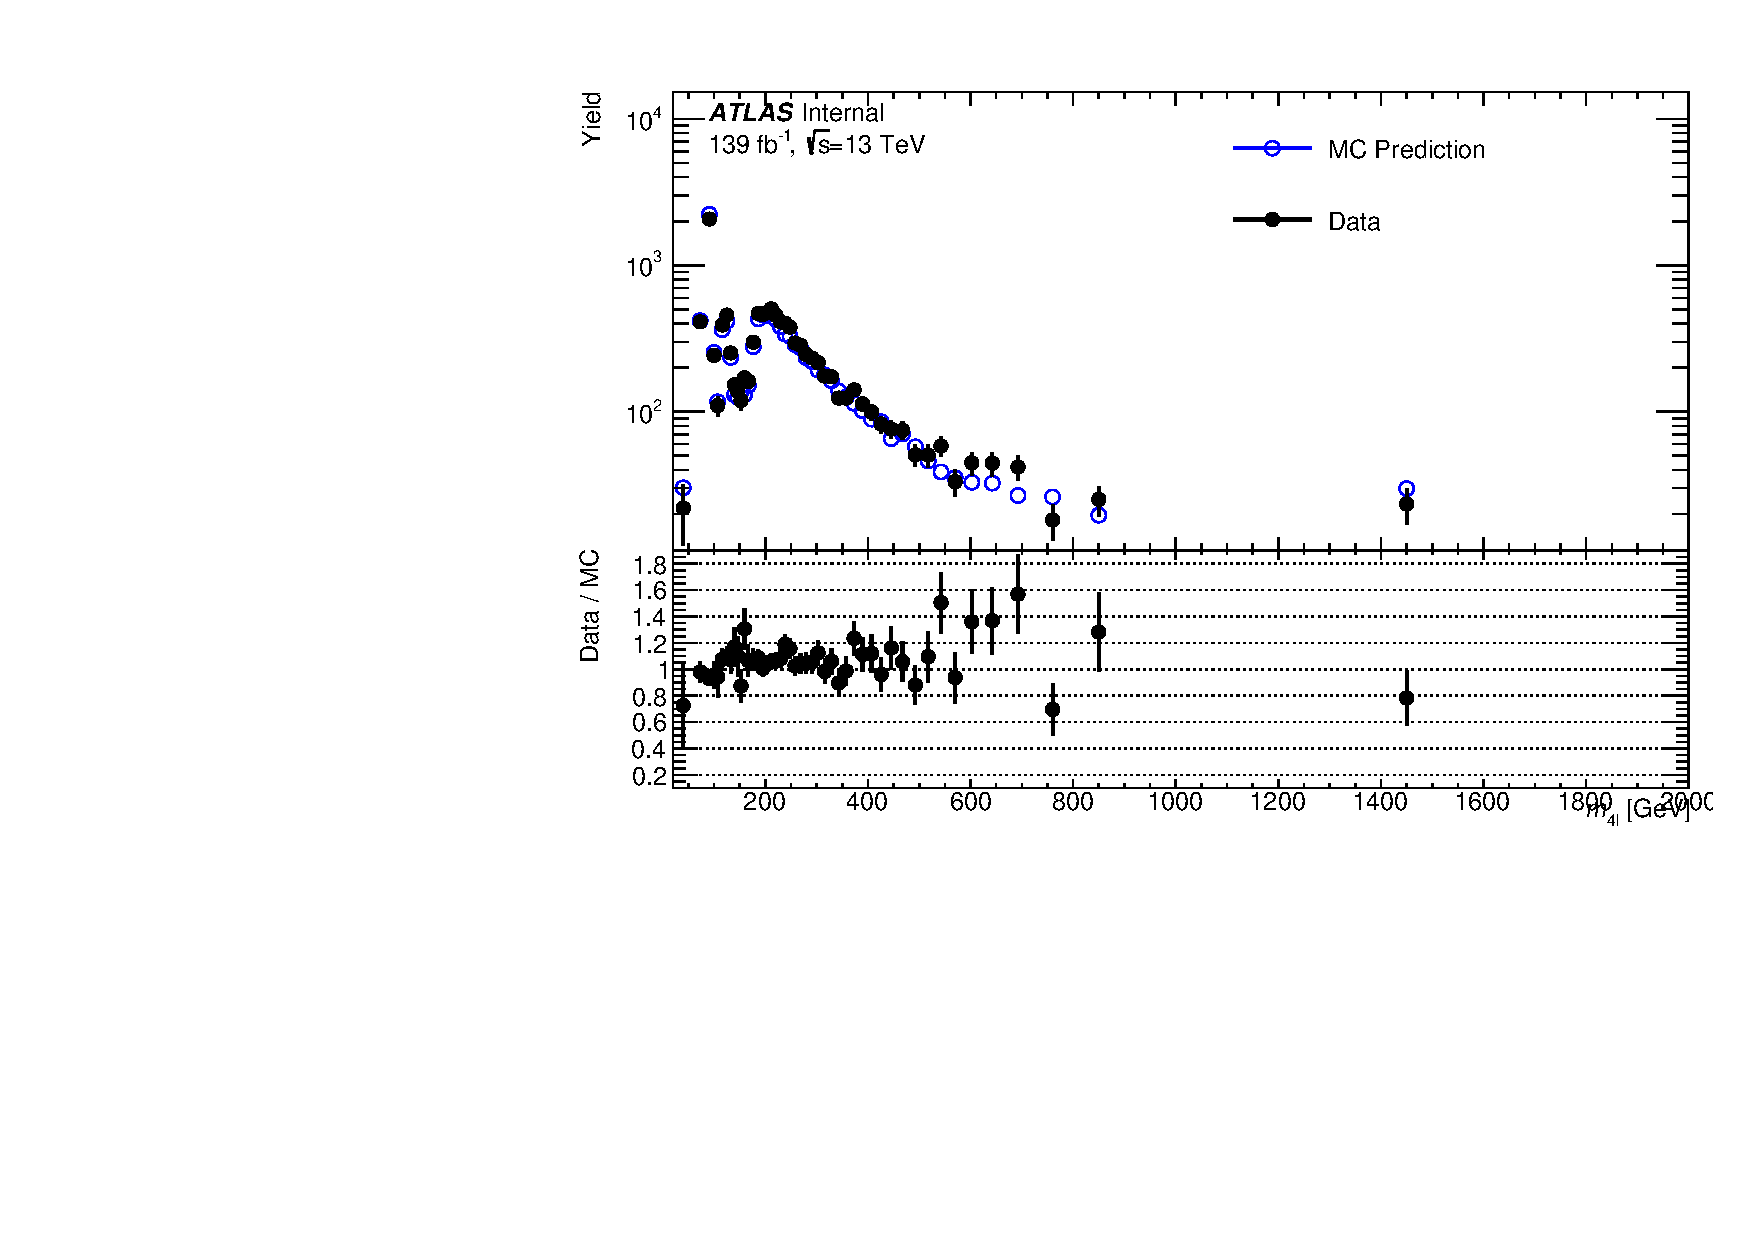
\includegraphics[width=.99\linewidth]{Figures/m4l/DataDriven/RatioM4l.pdf}\caption{}
    \end{subfigure}
    \begin{subfigure}{.49\textwidth}\centering
      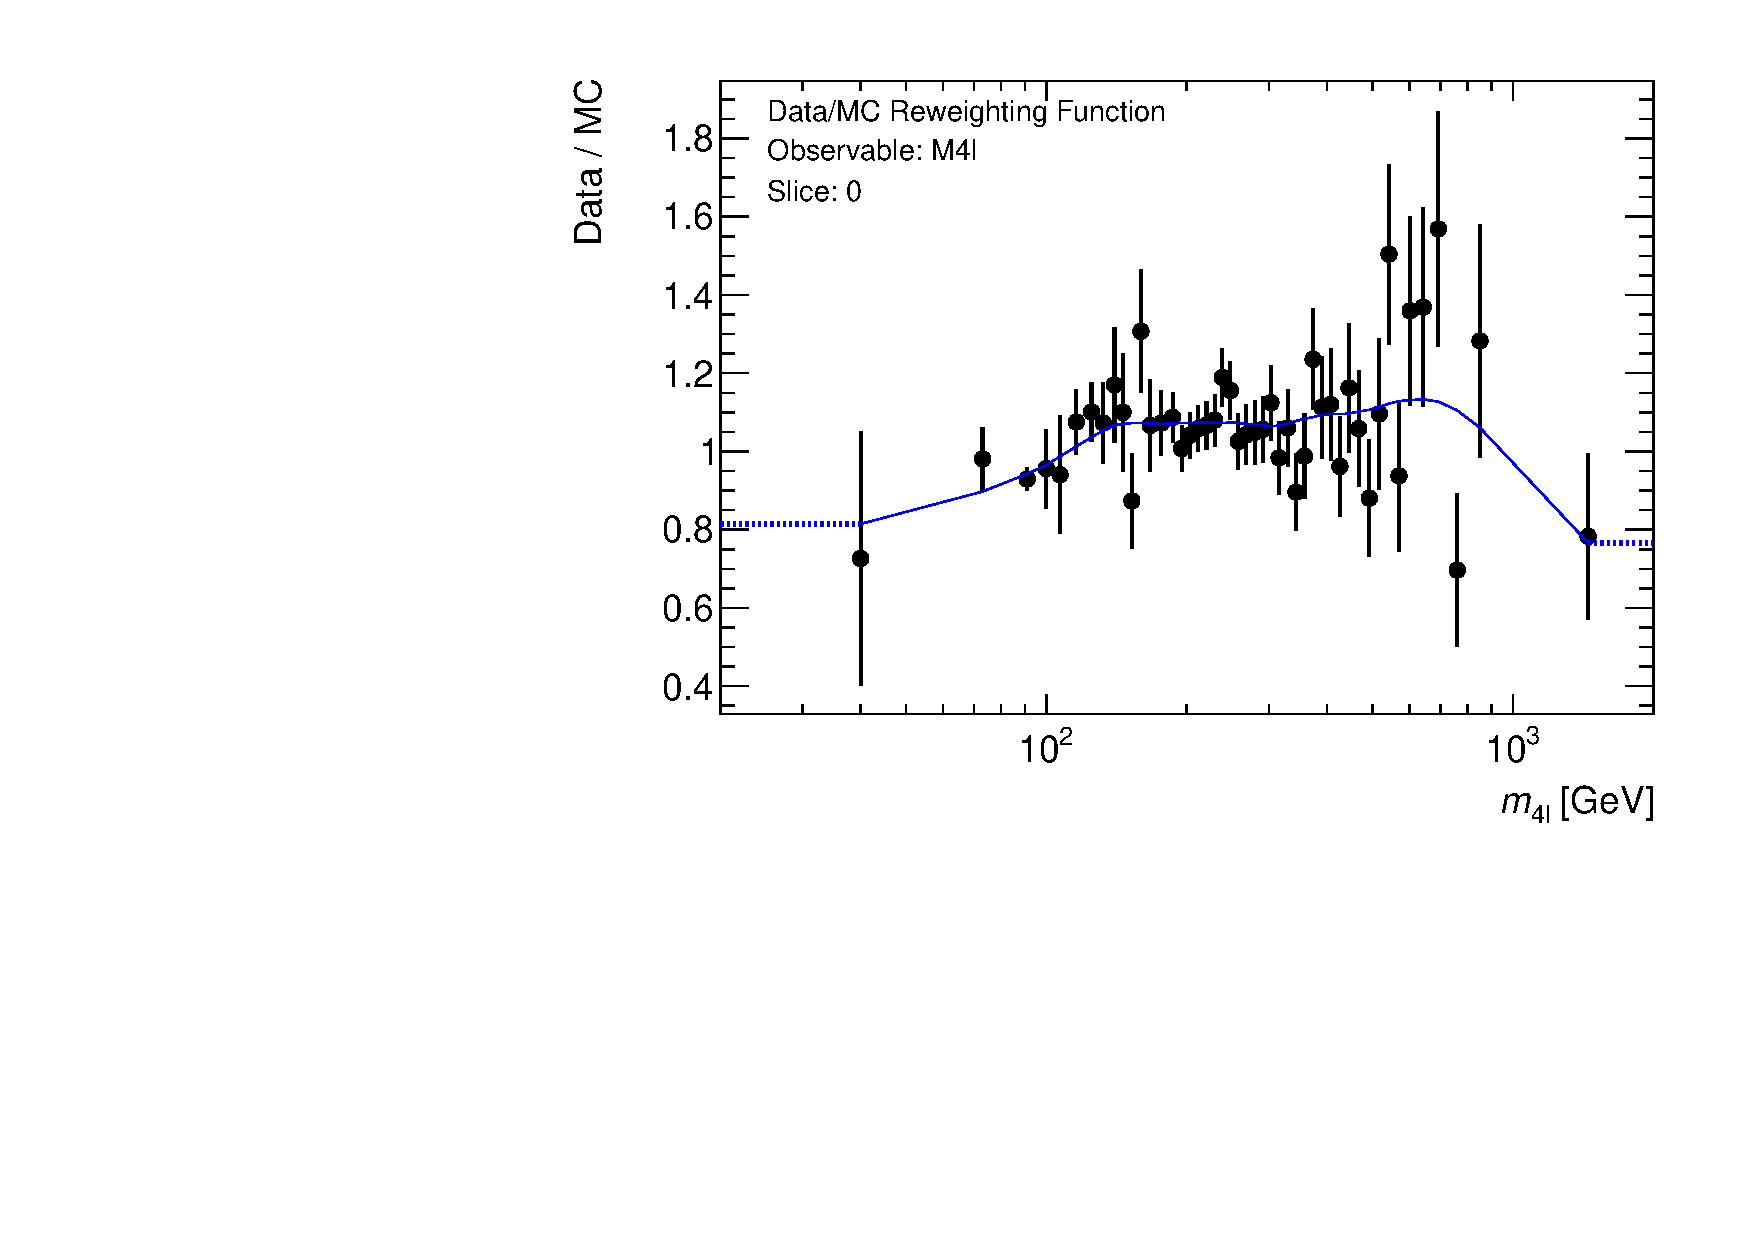
\includegraphics[width=.99\linewidth]{Figures/m4l/DataDriven/FitM4l-Slice0.pdf}
    \end{subfigure}
    \begin{subfigure}{.49\textwidth}\centering
      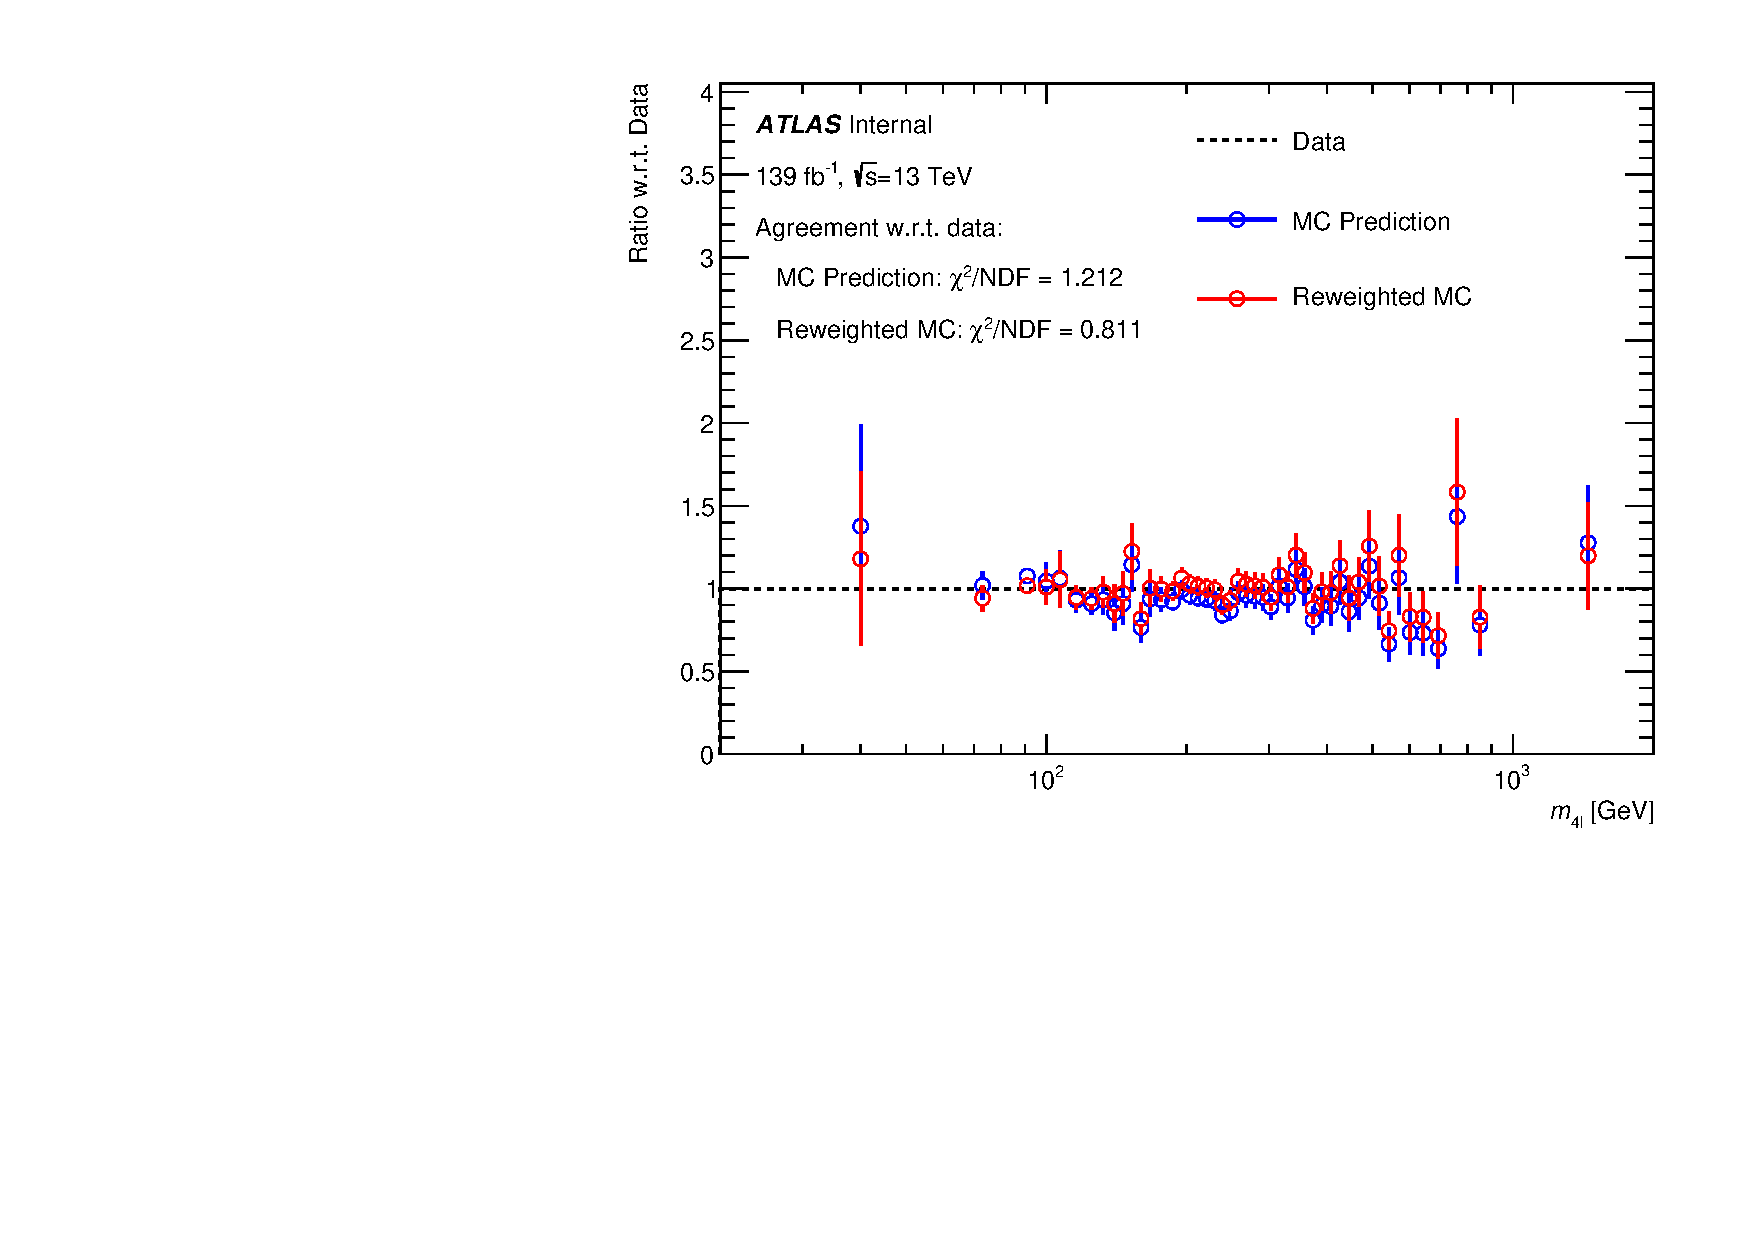
\includegraphics[width=.99\linewidth]{Figures/m4l/DataDriven/ReweightedM4l.pdf} 
    \end{subfigure}
    \begin{subfigure}{.49\textwidth}\centering
      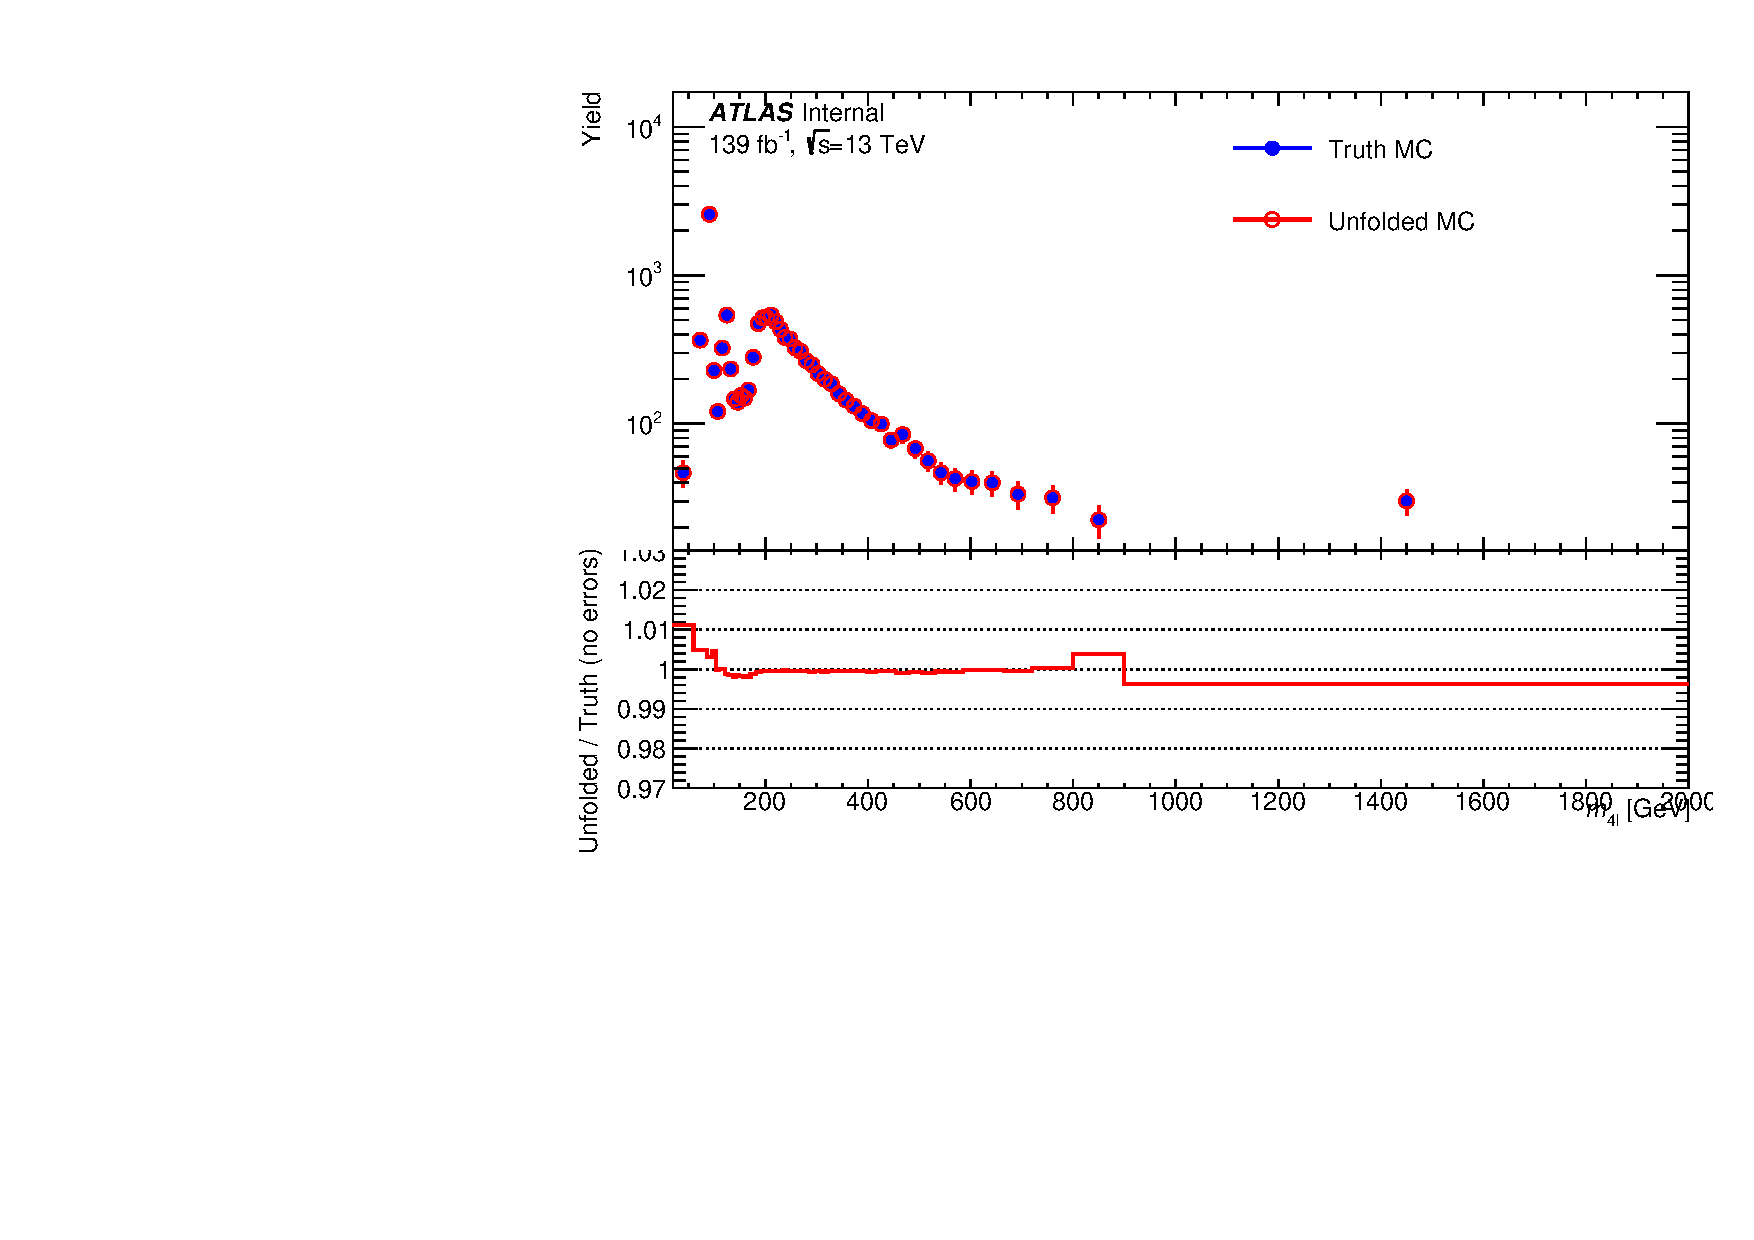
\includegraphics[width=.99\linewidth]{Figures/m4l/DataDriven/UnfoldedM4l.pdf}  
    \end{subfigure}
    \caption{Step-by-step overview of the data-driven method for $\mFourL$. In (a), the observed data is compared to the nominal SM MC prediction at reconstruction-level. In (b), the reweighting function is obtained via smoothing of the data/MC ratio and is fixed to its last value in the final bins, as shown by the dashed lines. In (c), the truth-reweighted MC is compared to the nominal MC at reconstruction-level, showing, as expected, an improved agreement with the data. In (d), the difference in the ratio from unity is taken as the relative systematic uncertainty. \label{fig:m4ldatadriven}}
\end{figure}

\subsection{Injection studies}
\label{ssec:injectiontests}
Section \ref{sec:closuretests} demonstrates that the unfolding procedure has closure when unfolding pseudodata that agree with the Standard Model. Since the SM predictions themselves were used to derive the corrections and matrix used for unfolding, this is the expected case. The shape of real data is unknown, however, and may be different than the Standard Model prediction. Should the \mFourL spectrum be host to contributions that differ from the SM prediction, it is necessary to check that the unfolding procedure is nonetheless able to provide an accurate and unbiased particle-level result. In order to do this a number of injection tests were performed. The first step is to take the nominal SM prediction, and inject some amount of BSM signal into it. The reconstruction level yield of this modified sample is used as pseudodata. It is run through the standard unfolding workflow in entirety, and compared to the particle level yield of the modified sample. Conceptually, this procedure is very similar to that of the Monte Carlo closure tests. 

A number of modifications were made to the nominal SM prediction, one set had the addition of a gluon-gluon fusion produced heavy Higgs boson with a mass of 300, 800, or \unit{1400}{\GeV} with either a narrow width or a width 15\% of its mass, and another set where the heavy Higgs was produced via vector-boson fusion. The \ggZZ process was also modified to have a larger event weight with respect to the SM prediction. These are described in full in Table \ref{tab:injectionsamples}. All of the models describe BSM scenarios with extremely large enhancements or resonances. 
\begin{table}
    \begin{tabular}{lll}
                            & Injection samples & \\
        \midrule \\
                            &               & 300 GeV \\
         Gluon-gluon fusion &  Narrow width & 800 GeV\\
                            &               & 1400 GeV \\
                            &               & 300 GeV \\
                            & 15\% width    & 800 GeV \\
                            &               & 1400 GeV \\
         \midrule \\
                                & & 300 GeV \\
         Vector-boson fusion    & & 800 GeV \\
                                & & 1400 GeV \\
         \midrule \\
         \ggZZ enhancement & \\
    \end{tabular}
  \caption{Modifications made to the nominal SM prediction for injection studies.}
  \label{tab:injectionsamples}
\end{table}
For each of the variations listed in Table \ref{tab:injectionsamples}, a range of cross-sections were injected and then unfolded with and without application of the pre-unfolding weights. In order to carve a more realistic scenario, one of the injected cross-sections for the heavy Higgs samples was set to be just within the two-sigma band of the data uncertainty. This was done by increasing the injected cross-section and calculating the $p$-value between the BSM prediction and the data until a $p$-value smaller than or equal to 0.05 is reached\footnote{This is the $p$-value corresponding to a two-sigma significance.}.
\begin{figure}
    \centering
    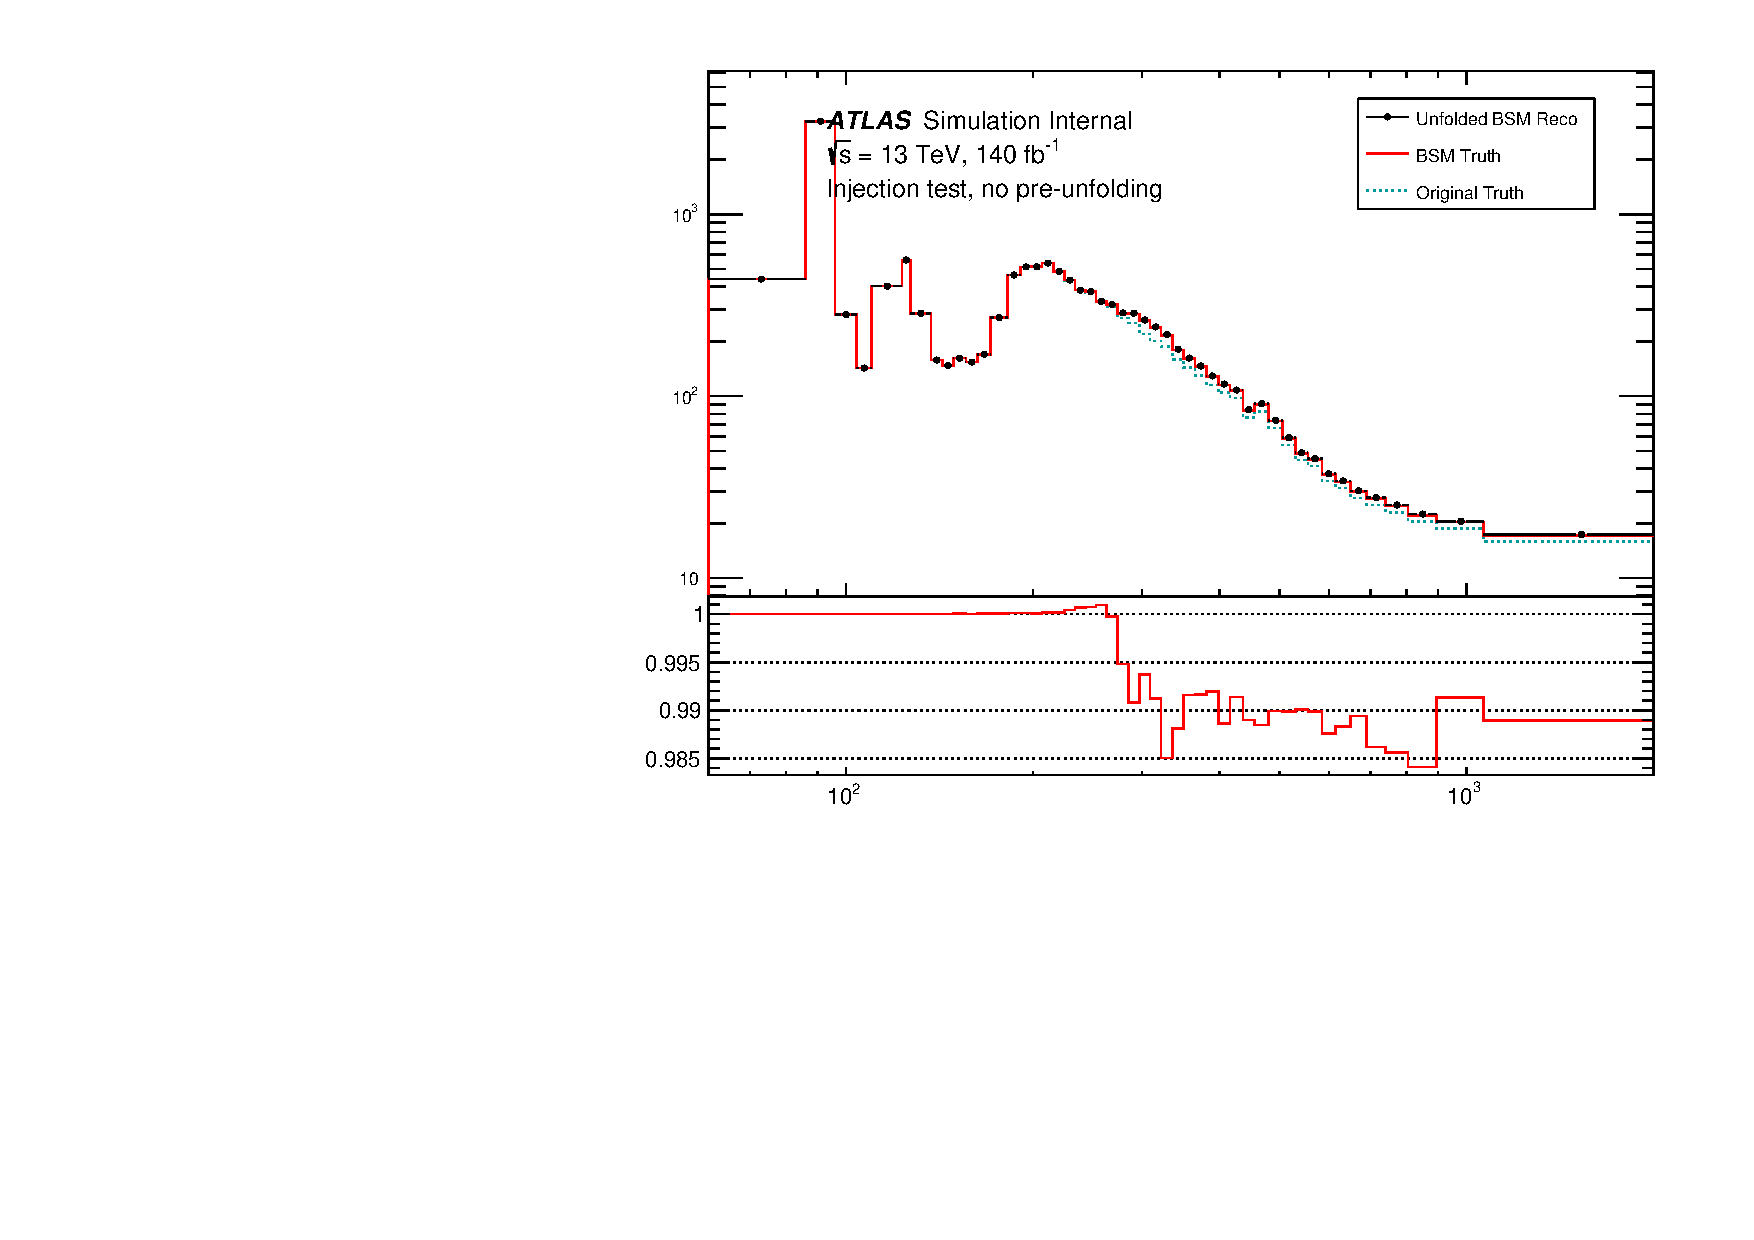
\includegraphics{Figures/m4l/InjectionTests/heavyH_unfolded.pdf}
    \caption{Caption}
    \label{fig:injectiontest}
\end{figure}
